\begin{frame}{Spezifikationen}
    \begin{exercise}[a) `Spezifikation' erfüllt?]
        Lies eine {\only<3>{\bfseries}Zahl} von der Tastatur ein, {\only<5>{\bfseries}berechne die Quadratwurzel}, und {\only<7>{\bfseries}gib das Ergebnis am Bildschirm aus}.
    \end{exercise}
    \pause[]
    \begin{solve}[a)]
    \begin{enumerate}
        \item Vollständig: \onslide<4-8>{Welche Zahlendarstellung? Negative Zahlen? \faTimes}
        \item Detailliert: \onslide<6-8>{Welche Grundoperationen sind erlaubt? \faTimes}
        \item Unzweideutig: \onslide<8>{Was heißt ,,ausgeben''? \faTimes}
    \end{enumerate}
    \end{solve}
\end{frame}
% copy to cleanup my code
\addtocounter{exercise}{-1}\addtocounter{solve}{-1}% reset counters
\begin{frame}{Spezifikationen}
    \begin{exercise}[b) `Spezifikation' erfüllt?]
        Berechne die Länge des Wortes als Binärzahl, und zwar in der Formulierung aus Aufgabe 4 von Übungsblatt 2.
    \end{exercise}
    \begin{solve}[b)]
    \begin{enumerate}
        \item Vollständig: \onslide<3-5>{\faCheck}
        \item Detailliert: \onslide<4-5>{mathematisch formales Maschinenmodell \faCheck}
        \item Unzweideutig: \onslide<5>{Turingmaschine \faCheck}
    \end{enumerate}
    \end{solve}
    \only<2-5>{\begin{tikzpicture}[overlay]
        \node[inner sep=0] (n0) at (current page.east) {};
        \only<2>{\node[below left = 3em and 2em of n0] (n1) {\begin{tcolorbox}[boxrule=0.1pt,hbox,boxsep=2pt,left=0pt,right=0pt,top=0pt,bottom=0pt]
            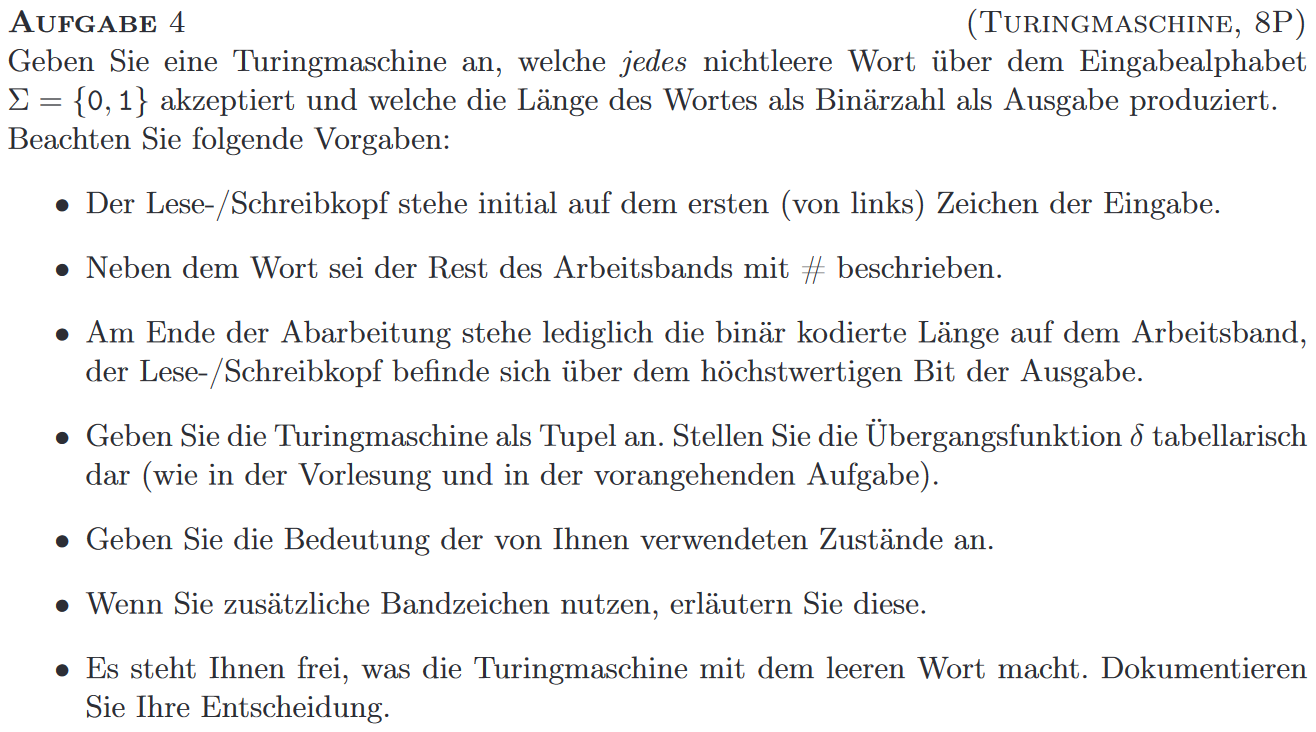
\includegraphics[scale=0.65]{sources/blatt2aufgabe4.png}
        \end{tcolorbox}};}
        \only<3-5>{\node[below left = -1.5em and 3em of n0] (n1) {\begin{tcolorbox}[boxrule=0.1pt,hbox,boxsep=2pt,left=0pt,right=0pt,top=0pt,bottom=0pt]
            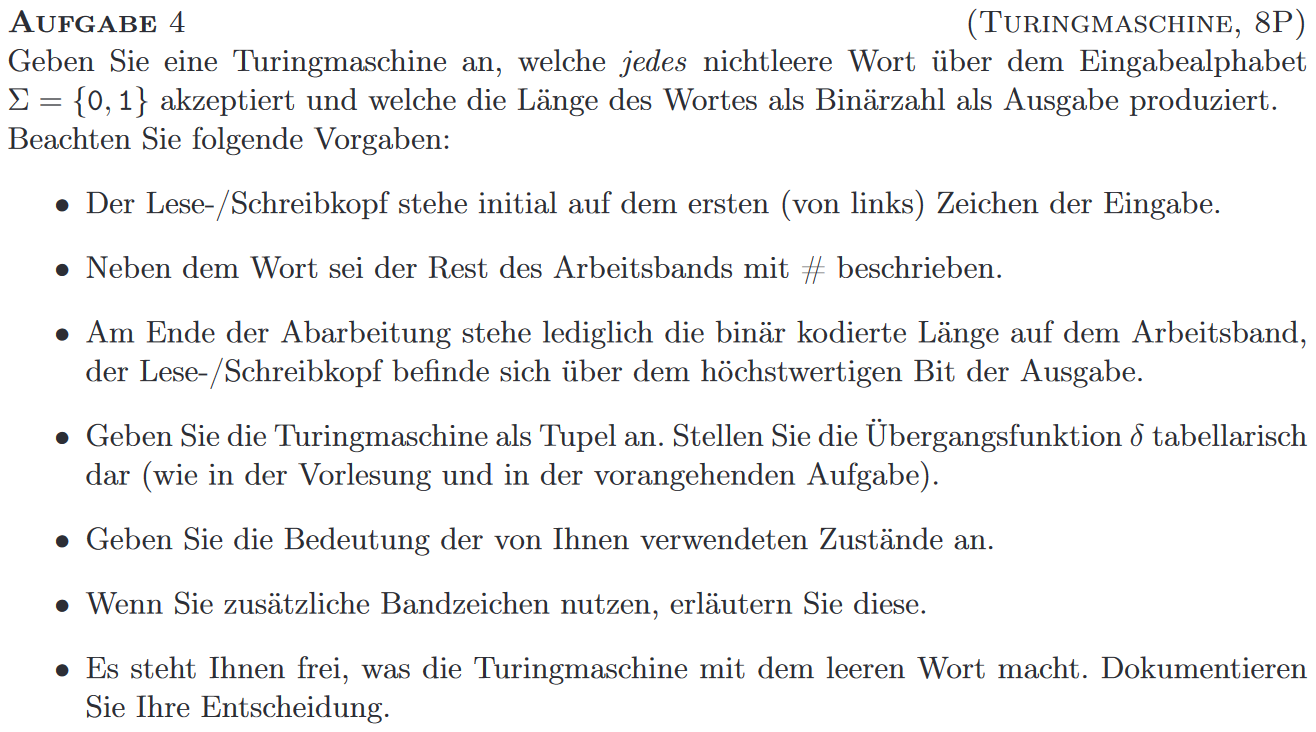
\includegraphics[scale=0.2]{sources/blatt2aufgabe4.png}
        \end{tcolorbox}};}
    \end{tikzpicture}}
\end{frame}